%%%%%%%%%%%%%%%%%%%%%%%%%%%%%%%%%%%%%%%%%%%%%%%%%%%%%%%%%%%%%%%%%%%%%%%%%%%%%%%%
%2345678901234567890123456789012345678901234567890123456789012345678901234567890
%        1         2         3         4         5         6         7         8
% THESIS CHAPTER

\chapter{Work Undertaken}

% short summary of the chapter
\section*{Measures}

\section{Final User Interface}

\begin{figure}[h!]
  \begin{center}
  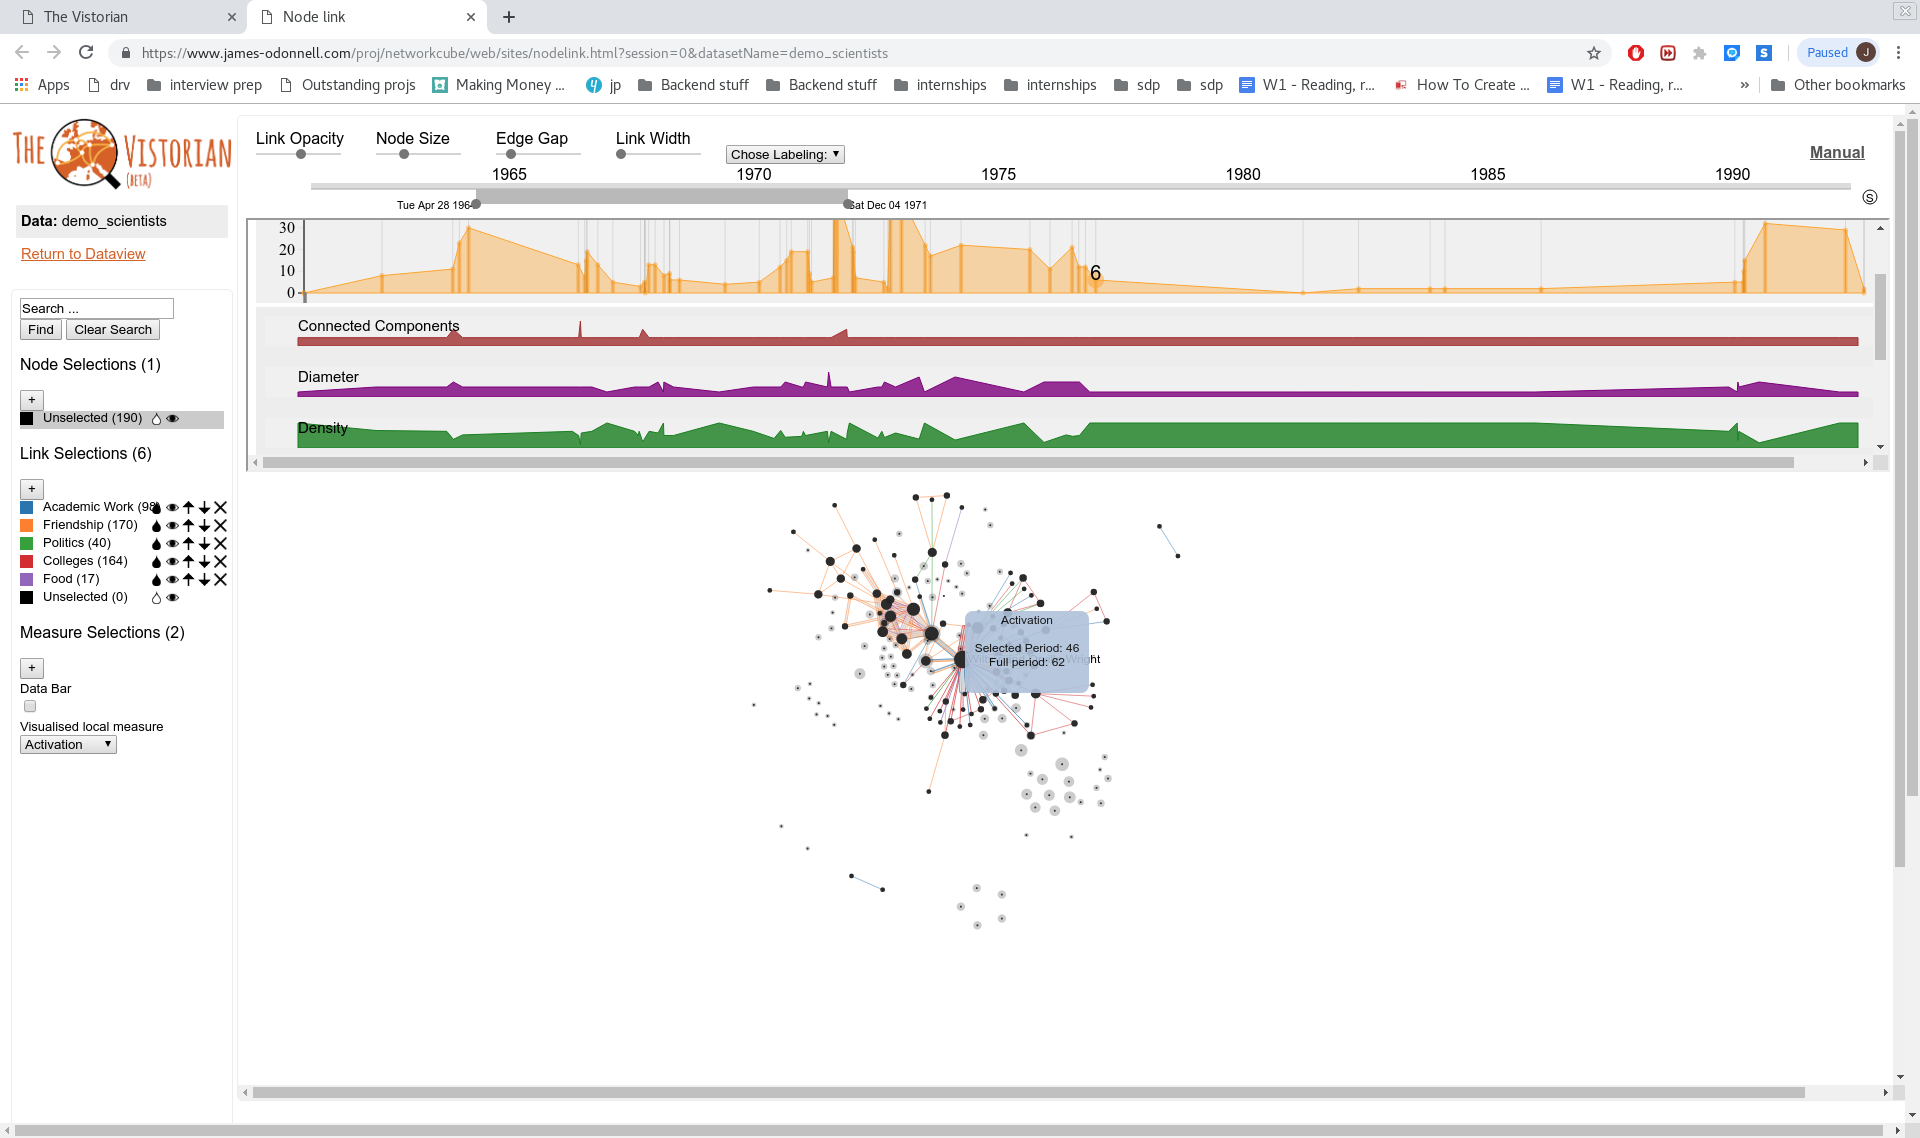
\includegraphics[trim={0, 0, 0, 3.5cm}, clip, width=140mm]{./Figures/vistorianNewFull.png}
  \caption{Full updated user interface}
  \label{fig:vistorianNewFull}
  \end{center}
\end{figure}

\subsection{The Databar}

\begin{center}
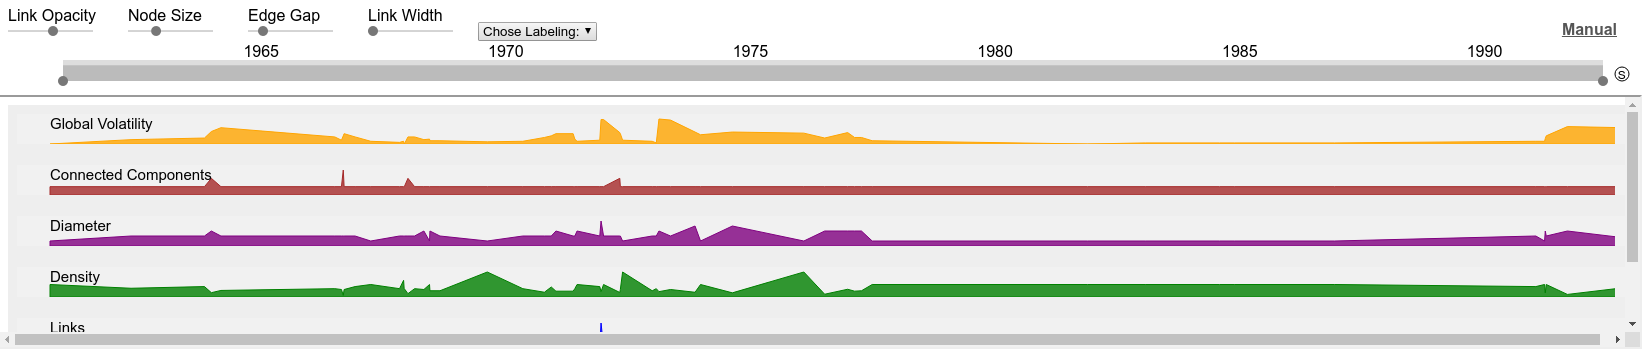
\includegraphics[trim={0 0 0 0}, width=140mm]{./Figures/databar.png}
\end{center}

The Databar holds the visualisation graphs for global measures. I decided to place it along the top of the window because it would line up nicely with the pre-existing timeline which could then double as the x-axis label - saving valuable screen space.
The databar is highly interactive. Each graph is initially collapsed and can then be expanded by clicking. As more measures were added I realised that it wouldn't be possible to both provide enough detail in every graph and also facilitate easy comparison without taking up most of the screen real estate. Collapsing and expanding the graphs solved this problem. The databar was designed to be readily extensible and only needs to be provided with a list of values the same length as the number of time frames. It then maps each value to the corresponding time frame to produce the co-ordinate values for the ridgeline. 

\begin{center}
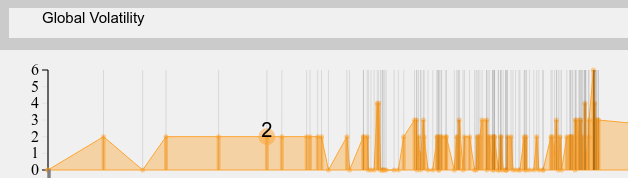
\includegraphics[trim={0 0 0 0}, width=140mm]{./Figures/margueriteGlobalVolatility.png}
\end{center}
A d3 scale is used to provide the y axis labels seen on the left of the expanded graph. Moving the mouse across the screen causes a cursor to track along the ridgeline of the graph. The y-label at that point is shown on the tracker. This was originally done when the graphs weren't expandable to remove the need for an axis and save space, however it was found to be useful for tightly clumped values and for data with some small step sizes.

\begin{center}
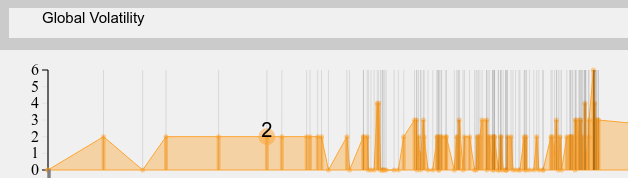
\includegraphics[trim={5cm, 0, 9cm, 2cm},clip, width=70mm]{./Figures/margueriteGlobalVolatility.png}
\end{center}
The vertical lines indicate a timestep/change in the graph. This was orignally simply intended to make it easier for the user to  compare graphs vertically, however an additional and powerful benefit is that it allows the user to  easily finding time periods of high or low activity. The vertical lines are thicker and of the same colour as the graph when inside it's area to emphasise the fact that these are the only points there is information for, and that the connecting ridge-line is interpolated between them.
Finally, graphs can be reordered for easy comparison using click and drag as there is not enough screen space to see all graphs at once, even compressed.

\subsection{Bookmarks Bar Additions}
\begin{figure}
  \begin{center}
  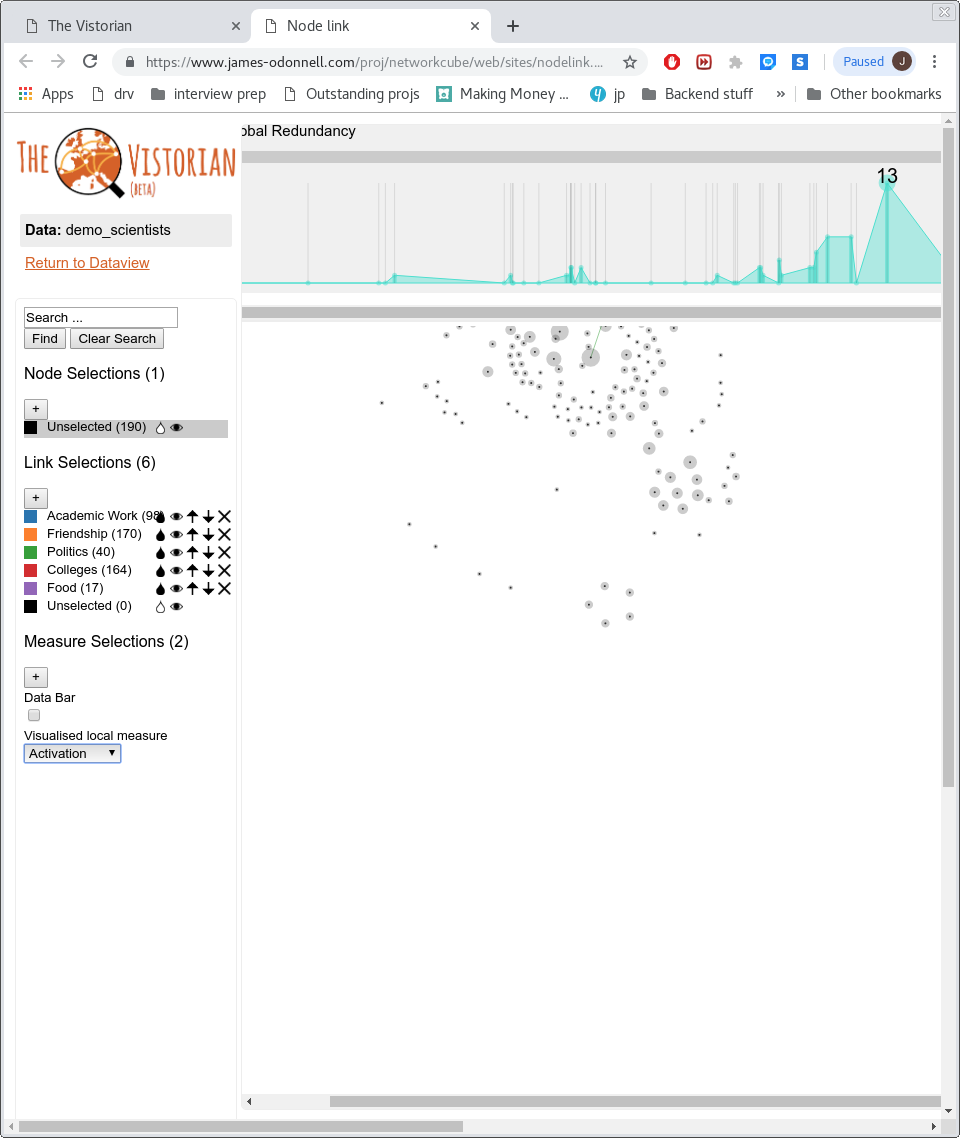
\includegraphics[trim={0, 12cm, 20cm, 22cm},clip, width=140mm]{./Figures/bookmarksbar.png}
  \caption{Bookmarks Bar Measures Extension}
  \label{fig:bookmarksbar}
  \end{center}
\end{figure}

The bookmarks bar has been extended with a checkbox to show or hide the databar and a dropdown to pick between local measures, shown in Figure \ref{fig:bookmarksbar}. It defaults to centrality.






\section{Measures and Visualisations}
The measures that have been implemented are each detailed below. The methods of calculation, the reasons for selecting them, their applications in The Vistorian and potential further applications are provided.

%%%%%%%%%%%%%%%%%%%%%%%%%%%%%%%%%%%%%%%%%%%%%%%%%%%%%%%%%%%%%%%%%%%%%%%%%%%%%%%%%%%%%%%%%%%%%%%%%%%%%%%%%%%%%%%
%NUMBER OF Nodepairs
%%%%%%%%%%%%%%%%%%%%%%%%%%%%%%%%%%%%%%%%%%%%%%%%%%%%%%%%%%%%%%%%%%%%%%%%%%%%%%%%%%%%%%%%%%%%%%%%%%%%%%%%%%%%%%%
\subsection{Number of Nodepairs}
%\subsubsection{Summary}
Simply the total number of active nodepairs in the network at a given time - a global static measure quantified at each time frame. It gives a quick idea of the degree of activity during a time frame.

%\subsubsection{Reasons for Selection}
The number of nodepairs is one of the most basic measures. However it aids understanding of the network considerably as it provides perhaps the simplest way of understanding the overall size of the network at a time frame or how it varies during a period, keeping cognitive load low while still improving understanding considerably.

%\subsubsection{Vistorian Implementation}
In The Vistorian this measure is interpreted as how the the number of connections varies over time, rather than the number of messages.


\begin{figure}[h!]
  \begin{center}
  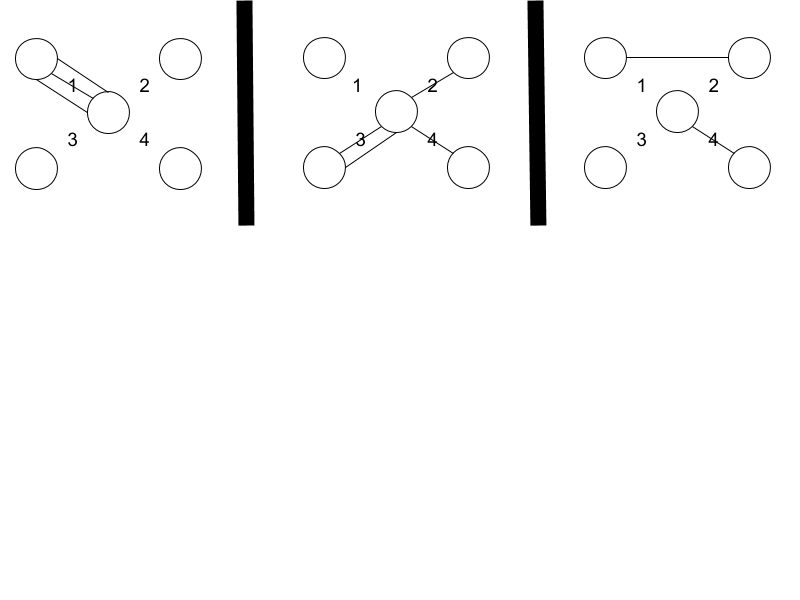
\includegraphics[trim={0 11cm 0 0}, clip, width=140mm]{./Figures/globalMeasuresReferenceNetwork.png}
  \end{center}
  \caption{Demonstration Network}
  \label{fig:demonstrationNetwork}
\end{figure}


In the demonstration network, Figure \ref{fig:demonstrationNetwork}, this measure would take the values [1, 3, 2]. Note that although there are 3 edges/messages in the first time frame there is only one nodepair.

%\subsubsection{Visualisation}                                                                                
%\subsubsection{Further Applications}


%%%%%%%%%%%%%%%%%%%%%%%%%%%%%%%%%%%%%%%%%%%%%%%%%%%%%%%%%%%%%%%%%%%%%%%%%%%%%%%%%%%%%%%%%%%%%%%%%%%%%%%%%%%%%%%
%NUMBER OF ACTIVE NODES
%%%%%%%%%%%%%%%%%%%%%%%%%%%%%%%%%%%%%%%%%%%%%%%%%%%%%%%%%%%%%%%%%%%%%%%%%%%%%%%%%%%%%%%%%%%%%%%%%%%%%%%%%%%%%%%
\subsection{Number of Active Nodes}
%\subsubsection{Summary}
Another global static measure. The number of active nodes is calculated as the total number of nodes with at least one edge in the network for each time frame.

%\subsubsection{Reasons for Selection}
Like the number of edges, the number of active nodes is also a very basic measure. However it gives an easily interpretable sense of the number of actors at a given time. Knowing if activity is high because there are multiple actors or because those actors are each very active is important to be able to distinguish. As it is a simple measure it also keeps cognitive load low while still improving understanding considerably.

%\subsubsection{Vistorian Implementation}
In the Vistorian this gives an idea of the number of people involved at each time frame, either sending or receiving messages. 
In the demonstration network, Figure \ref{fig:demonstrationNetwork}, this measure would take the values [2, 4, 4]. 

%\subsubsection{Visualisation}
%\subsubsection{Further Applications}

%%%%%%%%%%%%%%%%%%%%%%%%%%%%%%%%%%%%%%%%%%%%%%%%%%%%%%%%%%%%%%%%%%%%%%%%%%%%%%%%%%%%%%%%%%%%%%%%%%%%%%%%%%%%%%%
%DIAMETER
%%%%%%%%%%%%%%%%%%%%%%%%%%%%%%%%%%%%%%%%%%%%%%%%%%%%%%%%%%%%%%%%%%%%%%%%%%%%%%%%%%%%%%%%%%%%%%%%%%%%%%%%%%%%%%%
\subsection{Diameter}
%\subsubsection{Summary}
The longest of all shortest paths in the network at a given time. Diameter gives a sense of the interconnectedness of a network. A high diameter would mean the network is quite loose and linear, a low diameter implies nodes tend to be tightly connected with each other - however there could of course be a particularly long branch responsible for creating a high value which. Diameter is applied as a global static measure.

%\subsubsection{Reasons for Selection}
Diameter was selected as a measure because no other measure gives a sense of network breadth. It works particularly well alongside density to paint a picture of how the shape of the network evolves over time.
%Diameter is particularly important in social networks. The commonly known six-degrees of separation theory https://www.jstor.org/stable/pdf/2786545.pdf?acceptTC=true effectively states that if one were to make a social networks of all humans, the expected diameter would be 6. In a dynamic context... 

%\subsubsection{Vistorian Implementation}
In The Vistorian the diameter gives a sense of social distance or degrees of separation between individuals.
%\subsubsection{Visualisation}
%\subsubsection{Further Applications}

In the demonstration network, Figure \ref{fig:demonstrationNetwork}, this measure would take the values [1, 2, 1]. 

%%%%%%%%%%%%%%%%%%%%%%%%%%%%%%%%%%%%%%%%%%%%%%%%%%%%%%%%%%%%%%%%%%%%%%%%%%%%%%%%%%%%%%%%%%%%%%%%%%%%%%%%%%%%%%%
%DENSITY
%%%%%%%%%%%%%%%%%%%%%%%%%%%%%%%%%%%%%%%%%%%%%%%%%%%%%%%%%%%%%%%%%%%%%%%%%%%%%%%%%%%%%%%%%%%%%%%%%%%%%%%%%%%%%%%
\subsection{Density}
%\subsubsection{Summary}
Density here is defined as $\frac{2|NodePairs|}{|Nodes|\,(|Nodes|-1)}$. It gives a sense of connectedness at a given period of time. Only nodes with at least one edge are counted. Essentially, if every node is connected to every other node then density will be 1. Density is a global static measure.

%\subsubsection{Reasons for Selection}
Density is used as one of the measures because it gives the user an overview of how interconnected the graph is at a given point and how that varies over time. Since the goal is to provide as much information about the behaviour of the graph as possible using as few measures as possible it is important that information overlap from different measures is minimised. An overview of density can't be easily gathered from observing the graph and it can't be easily extrapolated from the other selected methods.

%\subsubsection{Vistorian Implementation}
We define an active node as node that has sent or received a letter during a time frame. In The Vistorian a density of 1 at a time frame means that every active node during that time frame has either sent or received a letter from every other active node.

In the demonstration network, Figure \ref{fig:demonstrationNetwork}, this measure would take the values [1, 0.5, 0.33]. 

%\subsubsection{Visualisation}

%\subsubsection{Further Applications}

%%%%%%%%%%%%%%%%%%%%%%%%%%%%%%%%%%%%%%%%%%%%%%%%%%%%%%%%%%%%%%%%%%%%%%%%%%%%%%%%%%%%%%%%%%%%%%%%%%%%%%%%%%%%%%%
%NUMBER OF CONNECTED COMPONENTS
%%%%%%%%%%%%%%%%%%%%%%%%%%%%%%%%%%%%%%%%%%%%%%%%%%%%%%%%%%%%%%%%%%%%%%%%%%%%%%%%%%%%%%%%%%%%%%%%%%%%%%%%%%%%%%%
\subsection{Number of connected components}
\subsubsection{Summary}
A connected component is a group of nodes connected by edges such that by traversing edges any node can be reached from any other node. This measure is simply the number of discrete connected components. It is a global static measure.

%\subsubsection{Reasons for Selection}
The number of connected components was selected as a measure because it shows how many distinct groups there are at any given point. The user could then step through the graph to see how these groups evolve over time.

%\subsubsection{Vistorian Implementation}
In The Vistorian, this measure can be interpreted as the number of distinct conversations happening during a given chunk of time. 

In the demonstration network, Figure \ref{fig:demonstrationNetwork}, this measure would take the values [1, 1, 2]. 

%\subsubsection{Visualisation}
%\subsubsection{Further Applications}

%%%%%%%%%%%%%%%%%%%%%%%%%%%%%%%%%%%%%%%%%%%%%%%%%%%%%%%%%%%%%%%%%%%%%%%%%%%%%%%%%%%%%%%%%%%%%%%%%%%%%%%%%%%%%%%
%CENTRALITY
%%%%%%%%%%%%%%%%%%%%%%%%%%%%%%%%%%%%%%%%%%%%%%%%%%%%%%%%%%%%%%%%%%%%%%%%%%%%%%%%%%%%%%%%%%%%%%%%%%%%%%%%%%%%%%%
\subsection{Centrality}
%\subsubsection{Summary}
Centrality here is a local measure. The specific implementation used is degree centrality \cite{degCent}. Degree centrality is simply the number of edges connected to a node in the given time period. It can be interpreted as static here despite being applied to a time-period rather than a time frame because it effectively treats that time-period as a fixed frame.

%\subsubsection{Reasons for Selection}
Degree centrality was implemented concretely in the project to complement the pre-existing visualisation - the size of nodes in the nodelink diagram in The Vistorian is fixed and proportional to the number of connected edges they have during the full time window. However since this changes for each time frame it's convenient to be able to read off the exact value, particularly for highly connected nodes with many links.

%\subsubsection{Vistorian Implementation}

%\subsubsection{Visualisation}
%\subsubsection{Further Applications}


%%%%%%%%%%%%%%%%%%%%%%%%%%%%%%%%%%%%%%%%%%%%%%%%%%%%%%%%%%%%%%%%%%%%%%%%%%%%%%%%%%%%%%%%%%%%%%%%%%%%%%%%%%%%%%%
%LOCAL VOLATILITY
%%%%%%%%%%%%%%%%%%%%%%%%%%%%%%%%%%%%%%%%%%%%%%%%%%%%%%%%%%%%%%%%%%%%%%%%%%%%%%%%%%%%%%%%%%%%%%%%%%%%%%%%%%%%%%%

\subsection{Local Volatility}

\subsubsection{Development}

In my literature review I didn’t come across any examples where this specific measure, or anything similar, was used or investigated. I felt that there needed to be some measure or score which captured the level of connection fluctuation such that a node whose connections tended to stay mostly within a fixed set of other nodes would score low but a node whose edges tended to be short lived and with unfamiliar nodes would score high. This was a highly experimental process as there are a number of ways this could be achieved.
Volatility is a local measure, calculate for a node and with respect to a set start time and end time. Initially it was calculated as the population standard deviation of the number of a node’s connections throughout that time period, effectively the variance in the number of connections.

\begin{center}
$N = total\ number\ of\ time\ frames$
$\overline{x} = average\ number\ of\ connections\ from\ given\ node $
$x_i = number\ of\ connections\ at\ time\ i$

$local\ volatility\ = \sqrt{\frac{1}{N} \sum_{i=1}^N (x_i - \overline{x})^2}$
\end{center}

Examples are given below, calculated for the central node.


\begin{center}
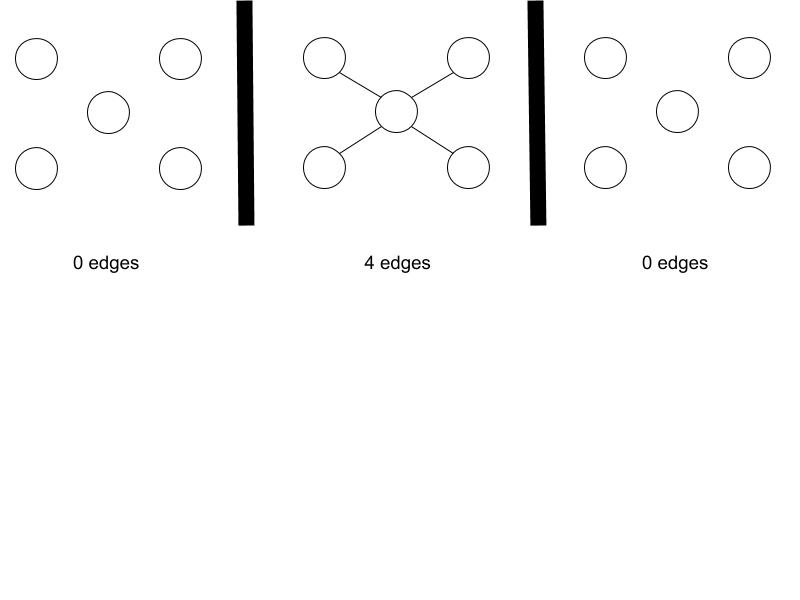
\includegraphics[trim={0 10cm 0 -1cm}, width=120mm]{./Figures/volatility1.jpg}

$N = 3$

$\overline{x} = \frac{4 + 0 + 0}{3} = \frac{4}{3}$

$local volatility =\frac{1}{3}\times((0 - \frac{4}{3})^2 + ((4 - \frac{4}{3})^2) + (0 - \frac{4}{3})^2) $

$local volatility = 1.89$

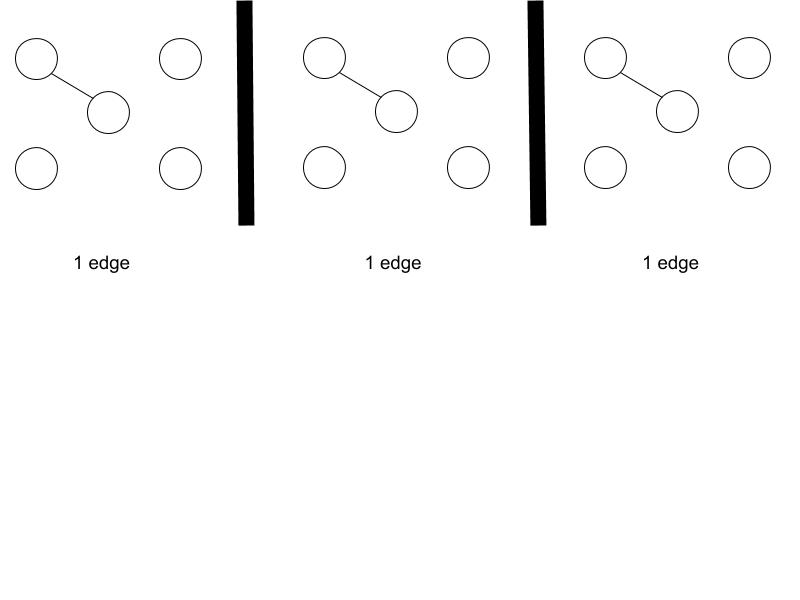
\includegraphics[trim={0 10cm 0 -1cm}, width=120mm]{./Figures/volatility2.jpg}

$N = 3$

$\overline{x} = \frac{1 + 1 + 1}{3} = 1$

$local volatility =\frac{1}{3}((1 - 1)^2 + ((1 - 1)^2) + (1 - 1)^2) $

$local volatility = 0$
\end{center}

Looking soley at these two examples this approach appears to work quite well - changes in edges results in a higher local volatility whereas no changes results in 0 local volatility.

However the problem with this approach is that it maintains no ‘memory’ of which edges were previously connected, consider the example below.
\begin{center}
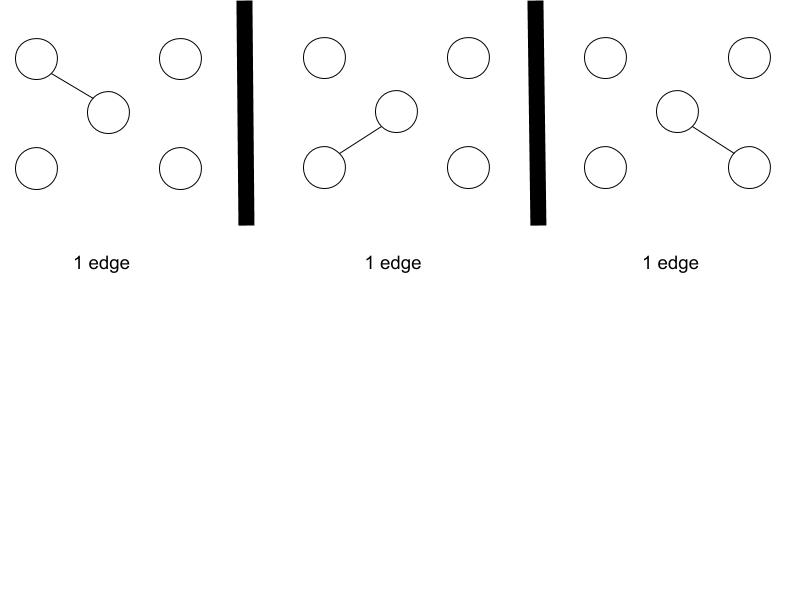
\includegraphics[trim={0 10cm 0 -1cm}, width=120mm]{./Figures/volatility3.jpg}
\end{center}

The local volatility will still be 0 despite the edge changing since only the number of edges is taken into account.

To fix this we must have some way to track individual edges, rather than solely the quantity. A solution is to give edges unique ids and store a binary value tracking which edges are present at each time frame and then sum the standard deviations of these. Example below, again calculated for the central node.

\begin{center}
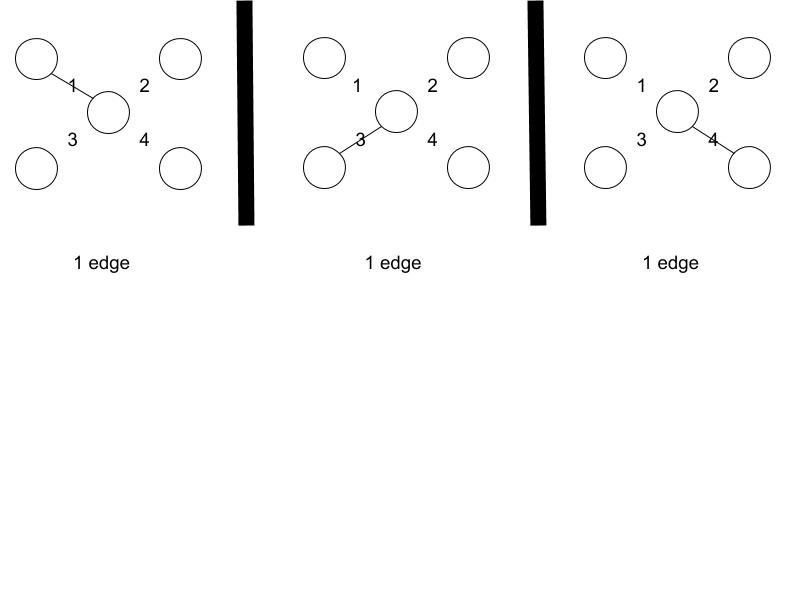
\includegraphics[trim={0 10cm 0 -1cm}, width=120mm]{./Figures/volatility4.jpg}
\end{center}

We store an object mapping as follows:

$edge\_id: [binary\ value\ indicating\ presence\ during\ timestep\ at\ index].$

\begin{center}
\{1:[1, 0, 0], 3: [0, 1, 0], 4: [0, 0, 1]\}
\end{center}
Local volatility could then be calculated as the average of the standard deviations of the object values.
\begin{center}
$local\ volatility = \frac{std([1,0,0]) + std([0,1,0]) + std([0,0,1])}{3}$

$local\ volatility = 0.47$
\end{center}

This approach too has an initially subtle problem however. Consider the figures below.
\begin{center}
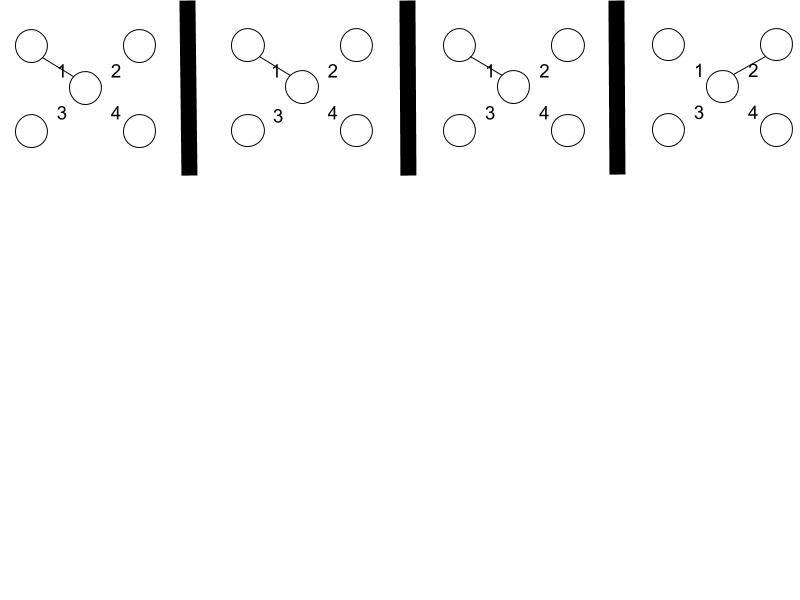
\includegraphics[trim={0 10cm 0 -1cm}, width=120mm]{./Figures/volatilityLastProblem1.jpg}
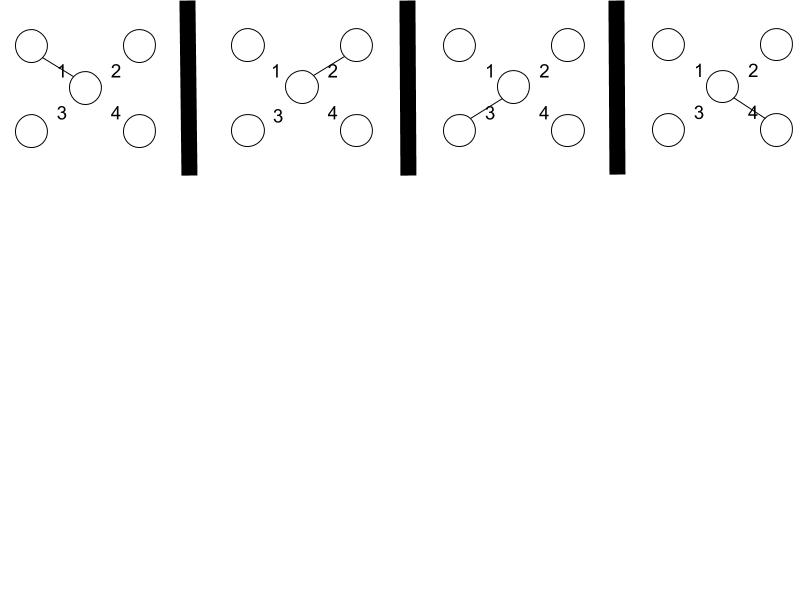
\includegraphics[trim={0 10cm 0 -1cm}, width=120mm]{./Figures/volatilityLastProblem2.jpg}
\end{center}
The volatility for the central node of the first network here would be calculated as follows.

\begin{center}
$N = 2$

$Mapping = \{1:[1, 1, 1, 0], 2:[0, 0, 0, 1]\}$

$local\ volatility = \frac{std([1,1,1,0]) + std([0,0,0,1])}{2}$

$local\ volatility = 0.43$
\end{center}

However upon calculating the volatility for the central node of the second network we find that it is equal. This is a problem because on observing the networks it can be seen that in network 1 there is a relatively stable edge, 1, for three of four time steps. Network 2 however has no edge lasting more than one time frame. This result does not align with the given specification of volatility, the second network should have a lower value than the first.

\begin{center}
$N = 4$

$Mapping = \{1:[1, 0, 0, 0], 2:[0, 1, 0, 0], 3: [0, 0, 1, 0], 4: [0, 0, 0, 1]\}$

$local\ volatility = \frac{std([1,0,0,0]) + std([0,1,0,0]) + std([0,0,1,0]) + std([0,0,0,1])}{4}$

$local\ volatility = 0.43$
\end{center}

The problem is caused by the averaging and the fact that the order of items does not affect standard deviation. My solution to this problem was to outright remove the averaging, and simply sum the terms. Since this could quickly lead to some very high values a log-scale is used for the visualisation. More details are provided on this in the visualisation method section \ref{sec:localMeasureVis}.  

With this fix the local volatility for the central node of the first network is 1.73 and 0.86 for the second network. 

To summarise, local volatility is calculated on a node. It is calculated as the cumulative sum of the standard deviations of the binary presences of each node that is present at least once in the given time frame.

Several more examples were worked through to ensure that volatility behaved as a user would expect given the way it is described, these are provided in Appendix \ref{appendix:appendixA}.

Since responsiveness is key, some space complexity is sacrificed. A large data structure is initialised on page load mapping nodes to nodepairs and nodepairs to their binary presence values at each time frame.
I considered further optimising by only storing positive presence values and extrapolating the negatives as needed for the standard deviation calculations, however this additional calculation would reduce responsiveness which is already somewhat limited in the browser.

\subsubsection{Vistorian Implementation}
Whilst this solution would work well in a general case it works poorly in The Vistorian as edges only appear once. To fix this we instead use node-pairs. 
Local volatility in The Vistorian gives a sense of the variation of a node's social contacts in a given time period. This is useful in the Vistorian because it allows us to see if one contact was rapidly sending or receiving messages to or from new contacts, or if they maintained fairly constant communication with a select number. 


\subsubsection{Further Applications}
Local volatility could have broad applications in other domains where dynamic networks are used. 
\newline\newline
Say a system administrator was conducting a post-mortem of an attack on a network using a dynamic network analysis tool to determine which nodes were potentially behaving maliciously. One measure useful in determining an anomaly in a network is the number of successfully established TCP connections in a time interval \cite{fnpfid}. A malicious port scan usually sends a relatively small number of packets to a large number of hosts on a network \cite{fnpfid}. If a similar volatility measure was implemented in this dynamic network analysis tool and TCP connections were considered to be edges it would be very easy for the system administrator to spot particularly volatile, or spiky, nodes.
\newline\newline
Whilst investigating different proteins in protein-protein interaction networks and their impact on the development and progression of hepatocellular carcinoma (HCC) after hepatitis C virus infection the protein core ESR1, which interacted with most of the nodes in the randomly selected sub-network, was shown to be associated with an increased HCC risk \cite{acaotdbnihih}. Using local volatility as a measure while performing this anaylsis would have immediately highlighted the ESR1 protein as highly volatile and worthy of further investigation.

%%%%%%%%%%%%%%%%%%%%%%%%%%%%%%%%%%%%%%%%%%%%%%%%%%%%%%%%%%%%%%%%%%%%%%%%%%%%%%%%%%%%%%%%%%%%%%%%%%%%%%%%%%%%%%%
%GLOBAL VOLATILITY
%%%%%%%%%%%%%%%%%%%%%%%%%%%%%%%%%%%%%%%%%%%%%%%%%%%%%%%%%%%%%%%%%%%%%%%%%%%%%%%%%%%%%%%%%%%%%%%%%%%%%%%%%%%%%%%

\subsection{Global Volatility}

%\subsubsection{Development}
To obtain some external feedback on the progress I had made an informal feedback meeting was held with with 4 active researchers on network analysis. These researchers were Dr Jim Lowe (James.Lowe@ed.ac.uk), Dr Miguel Garcia Sancho Sanchez (miguel.gsancho@ed.ac.uk), Mark Wong (Mark.Wong@glasgow.ac.uk) and Gil Viry (gil.viry@ed.ac.uk). I demonstrated usage of The Vistorian and the additions I had made for around 10 minutes, there was then around 15 minutes of discussion. In general there was a very positive reaction, which helped to validate the new additions. It was mentioned that a sense of overall volatility could be useful to complement the local volatility measure. This could be used to investigate if a node's local volatility was high simply because overall volatility was high or if it is worthy of further investigation. This became Global Volatility.

Global volatility is similar to local volatility in that it is a measure of change. It is defined as the change in active nodepairs for each time frame, starting from 0. If a nodepair wasn't active in the previous time frame but is active in the next then global volatility will be increased by one. Similarly if a nodepair was active in the previous time frame but wasn't active in the next then global volatility would also be increased by one as this is also a change. 

In figure \ref{fig:demonstrationNetwork2} this measure's values at each time frame would be [0, 4, 3]. The first time frame is 0 because there is no state beforehand to compare with, so it is treated as the base state. The second time frame is 4 because nodepair 1 is no longer active, and nodepairs 2,3 and 4 become active, summing to a total change of 4. For the final timeframe nodepairs 2 and 3 are lost and a new nodepair is added, summing to 3. Nodepair 4 is still active so it is not counted.

\begin{figure}[h!]
  \begin{center}
  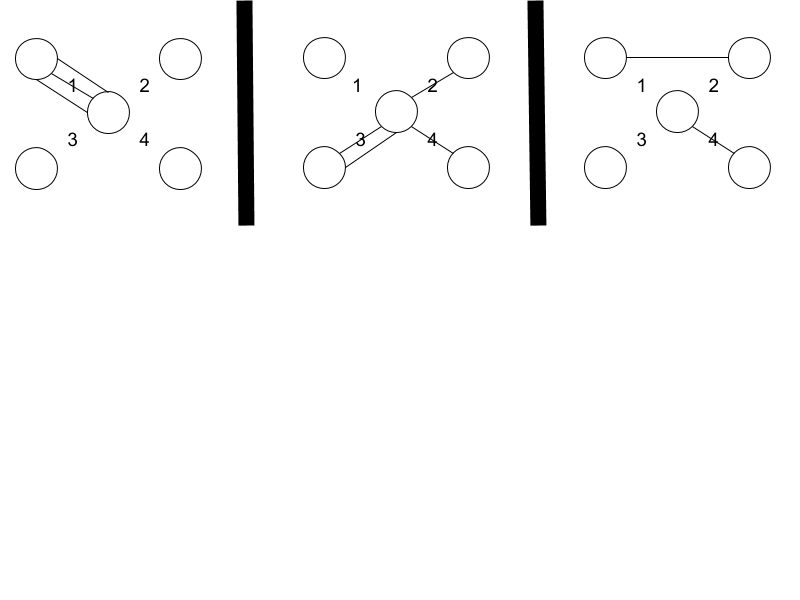
\includegraphics[trim={0 11cm 0 0}, clip, width=140mm]{./Figures/globalMeasuresReferenceNetwork.png}
  \end{center}
  \caption{Demonstration Network, repeated for convenience}
  \label{fig:demonstrationNetwork2}
\end{figure}


%\subsubsection{Vistorian Implementation}

%\subsubsection{Visualisation Method}

%\subsubsection{Further Applications}


%%%%%%%%%%%%%%%%%%%%%%%%%%%%%%%%%%%%%%%%%%%%%%%%%%%%%%%%%%%%%%%%%%%%%%%%%%%%%%%%%%%%%%%%%%%%%%%%%%%%%%%%%%%%%%%
%GLOBAL ACTIVATION
%%%%%%%%%%%%%%%%%%%%%%%%%%%%%%%%%%%%%%%%%%%%%%%%%%%%%%%%%%%%%%%%%%%%%%%%%%%%%%%%%%%%%%%%%%%%%%%%%%%%%%%%%%%%%%%

\subsection{Global Activation}
Global activation is a global dynamic measure. It is defined at each frame as the cumulative count of the number of new nodes that have been added, meaning that it will initialise as the number of nodepairs in the first frame, and end as the total number of nodes at the last frame. Observing this measure gives a sense of the rate at which new nodes are added. 

In The Vistorian, if global activation rapidly peaked and then only slowly climbed to the maximum but we also knew that activity was fairly constant this would imply that few new actors are added throughout the period and that most of the activity is between actors that have sent or received messages before.

In figure \ref{fig:demonstrationNetwork2} this measure's values at each time frame would be [1, 4, 5]. There is one nodepair in the first time frame, three previously unseen nodepairs are added in the second time frame - which brings the cumulative count to four, then one more unseen nodepair is added in the final frame.

%\subsubsection{Development}


%%%%%%%%%%%%%%%%%%%%%%%%%%%%%%%%%%%%%%%%%%%%%%%%%%%%%%%%%%%%%%%%%%%%%%%%%%%%%%%%%%%%%%%%%%%%%%%%%%%%%%%%%%%%%%%
%GLOBAL REDUNDANCY
%%%%%%%%%%%%%%%%%%%%%%%%%%%%%%%%%%%%%%%%%%%%%%%%%%%%%%%%%%%%%%%%%%%%%%%%%%%%%%%%%%%%%%%%%%%%%%%%%%%%%%%%%%%%%%%

\subsection{Global Redundancy}
Global redundancy is a global dynamic measure and is linked with global activation. It is defined as the number of nodes at each time frame that have been active in any previous time frame. Observing this measure gives a sense of the number of repeated nodes. A low redundancy implies that most nodes are only fairly inactive. A high redundancy implies that nodes are more active and reconnect often.

In figure \ref{fig:demonstrationNetwork2} this measure's values at each time frame would be [0, 0, 1]. This is because nodepair 4 is active in the second frame and then again in the final frame, so it is counted as redundant in the final frame.


%\subsubsection{Development}


%%%%%%%%%%%%%%%%%%%%%%%%%%%%%%%%%%%%%%%%%%%%%%%%%%%%%%%%%%%%%%%%%%%%%%%%%%%%%%%%%%%%%%%%%%%%%%%%%%%%%%%%%%%%%%%
%LOCAL ACTIVATION
%%%%%%%%%%%%%%%%%%%%%%%%%%%%%%%%%%%%%%%%%%%%%%%%%%%%%%%%%%%%%%%%%%%%%%%%%%%%%%%%%%%%%%%%%%%%%%%%%%%%%%%%%%%%%%%

\subsection{Local Activation}

Pascal Cristofoli (pascal.cristofoli@ehess.fr) [...]. Experimented with the new additions. He suggested two new measures be added as he often found himself calculating them manually. These measures are local activation and local redundancy.

Local Activation is a local dynamic measure. It is calculated as the number of connections in the selected time period that weren't ever active before that time period began. In the network below, Figure \ref{localActivation1}, if the four time frames represent the full time period, the local activation value for the central node would be 3. If the selected time period was from the second to final time frames, inclusive, then the activation value for the central node would be 2.

\begin{figure}[h!]
  \begin{center}
  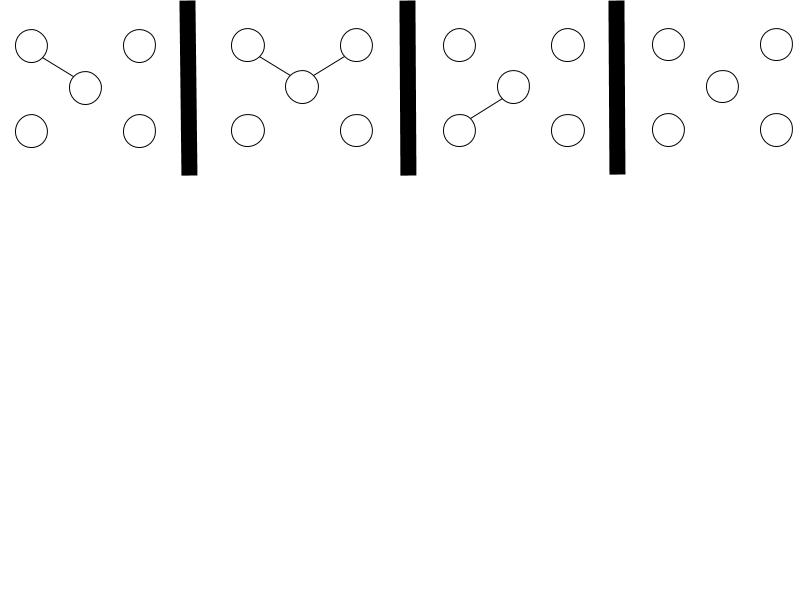
\includegraphics[trim={0 10cm 0 -1cm}, width=120mm]{./Figures/localActivation1.jpg}
  \end{center}
  \caption{}{}
  \label{localActivation1}
\end{figure}

%\subsubsection{Further Applications}
%Local activation could have broad applications in other domains where dynamic networks are used. 
%\newline\newline


%%%%%%%%%%%%%%%%%%%%%%%%%%%%%%%%%%%%%%%%%%%%%%%%%%%%%%%%%%%%%%%%%%%%%%%%%%%%%%%%%%%%%%%%%%%%%%%%%%%%%%%%%%%%%%%
%LOCAL REDUNDANCY
%%%%%%%%%%%%%%%%%%%%%%%%%%%%%%%%%%%%%%%%%%%%%%%%%%%%%%%%%%%%%%%%%%%%%%%%%%%%%%%%%%%%%%%%%%%%%%%%%%%%%%%%%%%%%%%

\subsection{Local Redundancy}

Local Redundancy is also a local dynamic measure, highly complementary to local activation. It is calculated as the number of connections in the selected time period that have been active before that time period began. In the network above, Figure \ref{localActivation1}, if the four time frames represent the full time period, the local redundancy value for the central node would be 0, since there are no prior connections. If the selected time period was from the second to final time frames, inclusive, then the redundancy value for the central node would be 1.

\subsubsection{Further Applications}
Local activation could have broad applications in other domains where dynamic networks are used. 
\newline\newline
%In 2002 a study was conducted using a network of business connections to investigate if the degree of redundancy in social networks influenced the success of business start-ups \cite{socRed}. Redundancy here is applied in a static sense, such that "In non‐redundant networks the entrepreneurs’ contacts do not know each other and rarely have the same information". If a dynamic network was used instead, and the local redundancy measure was applied then .... STATIC V DYNAMIC A BIT DIFFICULT HERE BUT I THINK IT COULD BE A GOOD ADDITION?

%%%%%%%%%%%%%%%%%%%%%%%%%%%%%%%%%%%%%%%%%%%%%%%%%%%%%%%%%%%%%%%%%%%%%%%%%%%%%%%%%%%%%%%%%%%%%%%%%%%%%%%%%%%%%%%
%LOCAL MEASURE VISUALISATION.
%%%%%%%%%%%%%%%%%%%%%%%%%%%%%%%%%%%%%%%%%%%%%%%%%%%%%%%%%%%%%%%%%%%%%%%%%%%%%%%%%%%%%%%%%%%%%%%%%%%%%%%%%%%%%%%
\section{Local Measure Hoverover}
\label{sec:localMeasureVis}
To save screen space and reduce visual complexity, the precise values of a node's local measures given the selected time period are only shown on hover over. For the purposes of this report, the local measures are degree centrality and local volatility. However the implementation is easily extensible, allowing for more local measures to be quickly visualised.

Initially, local volatility was visualised using 'spikes', where more spikes indicated higher local volatility. Other methods were considered, vibration matches with the mental image of volatility but would be too distracting to the eye. Dotted rings with larger diameter indicating higher local volatility were considered but had too much potential for confusing overlap. Colours were originally used but could be misconstrued as relating to the edge colours. 
However as more local measures were added the spikes made less sense. They were also somewhat difficult to count on smaller nodes.

\begin{center}
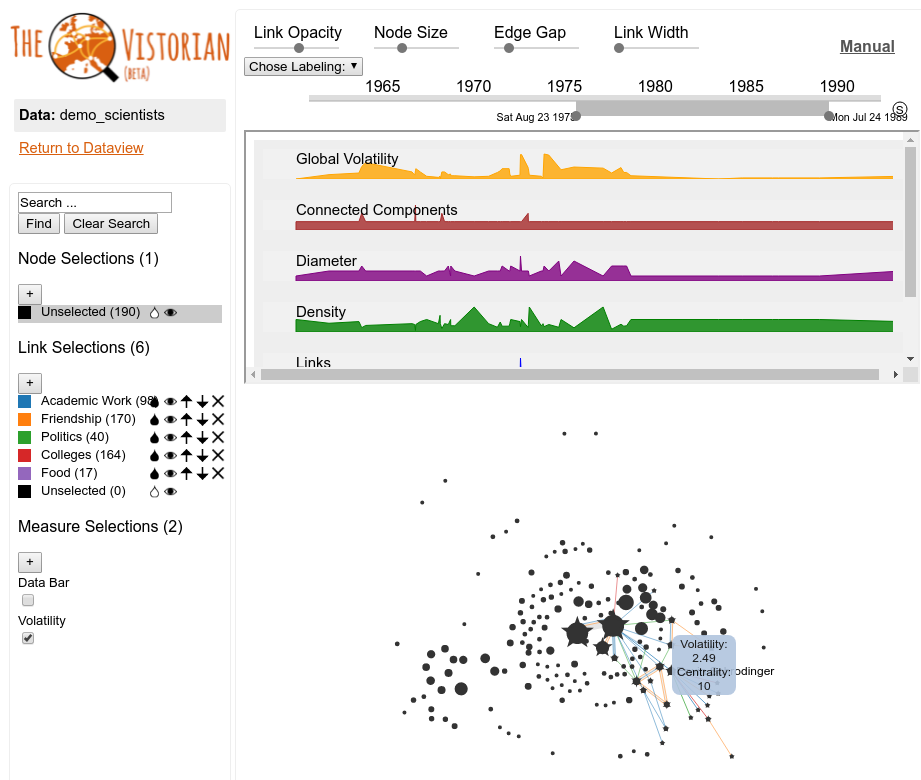
\includegraphics[trim={9cm, 0, 0, 14cm}, clip, width=140mm]{./Figures/finalUI.png}
\end{center}

Local activation, redundancy, volatility and centrality are all visualised in the same way - as the radius of the node in the network visualisation. The drop down in the bookmarks bar is used to select between them. The values are calculated for each node and the nodes radius is then calculated as the log of double the measures value, plus one. The values are doubled to give more visual separation which is hampered by the log scale. The "+1" is added so that nodes always have a radius to avoid breaking the user's mental map \cite{BLANK}.

To aid the user further, a lighter grey circle of a fixed radius is shown behind each node acting as a ghost. It's radius is calculated given the active local measure as that measures value over the full time frame. This allows users to see how a smaller window of time differs from the full time period. It was considered to use the maximum value that the selected measure ever takes for each given node, however this would require considerable initial computation as all pairs of start and end times would have to be considered for every single node. This solution doesn't work for redundancy as there are no redundant nodes over the full period.

\begin{figure}[h!]
  \begin{center}
  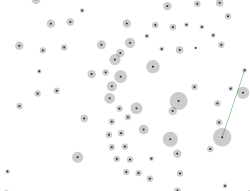
\includegraphics[trim={0, 0, 0, 0}, width=70mm]{./Figures/greyCircles.png}
  \caption{Fixed Ghost Nodes}
  \label{fig:greyCircles}
  \end{center}
\end{figure}



